\chapter{Algoritmi Greedy}
Si tratta di una tecnica che si applica sempre ai problemi di ottimizzazione, ma
rispetto alla programmazione dinamica ha un approccio diverso, dato che il calcolo della
soluzione ottima (in questo caso ne calcola una sola) avviene attraverso una
sequenza di scelte \textbf{localmente} ottime.
\paragraph*{Caratteristiche degli algoritmi Greedy}
\begin{itemize}
    \item Semplici da scrivere
    \item Efficienti
\end{itemize}
\paragraph*{Questioni}
\begin{itemize}
    \item Dimostrare la correttezza di un algoritmo greedy
    \item Capire quali problemi sono affrontabili con una strategia greedy
\end{itemize}
\section{Problema - Selezione attività}
\paragraph*{INPUT} Dato un insieme $A = \{a_1, a_2, \dots, a_n\}$ di n attività, tale
che $a_i = [s_i, e_i)$ per $\ \leq i \leq n$, dove $s_i$ è il tempo di inizio ed $e_i$ è il
tempo di fine.
\begin{center}
    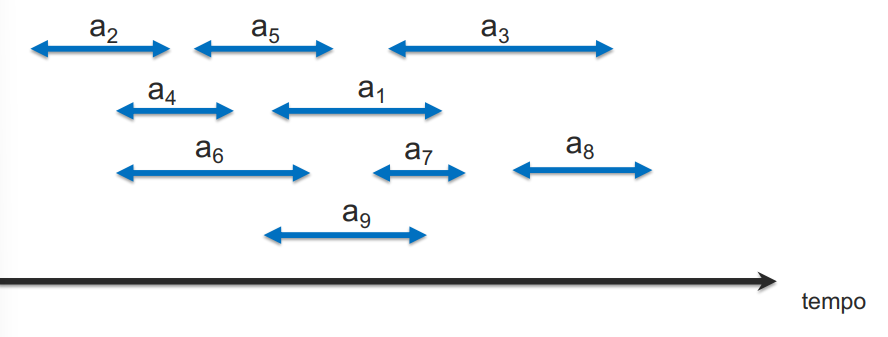
\includegraphics[width=80mm,scale=0.5]{greedy_sel_attivit.png}
\end{center}
$a_i=[s_i, e_i)$ e $a_j = [s_j, e_j)$ sono \textbf{compatibili} se $s_i \geq e_j$ oppure 
$s_j \geq e_i$. In poche parole se un attività inizia nello stesso momento della fine dell'altra, oppure dopo.
Le attività non devono accavallarsi, cioè eseguirsi nello stesso tempo di un'altra.
Facciamo qualche esempio che sicuramente è più semplice.\\
Per esempio $a_5=[s_5, e_5)$ e $a_8 = [s_8, e_8)$ sono compatibili, mentre $a_5 = [s_5, e_5)$ e 
$a_1 = [s_1, e_1)$ NON sono compatibili, infatti l'inizio di $a_1$ è minore della fine di $a_5$.
\paragraph*{OUTPUT} il sottoinsieme X di cardinalità massima composto di attività mutuamente compatibili.
In questo esempio l'OUTPUT desiderato è $X = \{a_2, a_5, a_7, a_8\}$.
\subsection{Soluzione con DP}
$A = \langle a_1, a_2,\dots,a_n\rangle$ tale che $e_1 \leq e_2 \leq \dots \leq e_n$.\\
$A = A \cup \{a_0, a_{n+1}\} = \langle a_0, a_1, \dots, a_n, a_{n+1}\rangle$ tale che $e_0 \leq s_1$
e $s_{n+1} \geq e_n$.
\paragraph*{Sottoproblema (i,j) per $0 \leq i < j \leq n+1$}
Trovare il sottoinsieme $X_{ij}$ di attività mutuamente compatibili di cardinalità massima per
$A_{ij} = \langle a_{i+1}, a_{i+2},\dots,a{j-2}, a{j-1} \rangle$.
\paragraph*{Sottoproblema $(0, n+1)$}
Trovare il sottoinsieme $X_{0,n+1} = X$ di attività mutuamente compatibili di cardinalità
massima per $A_{0,n+1} = \langle a_1, a_2, \dots, a_{n-1}, a_n \rangle = A$.\\
Numero totale di sottoproblemi \ra $(n+1)+n+(n-1)+(n-2)+\dots+1$.
\paragraph*{CASI BASE per $j=i+1 (A_{ij}=\emptyset)$}
$X_{ij} = \emptyset$.
\paragraph*{PASSO RICORSIVO per $j > i +1 (A_{ij} \neq \emptyset)$}
\textbf{Sottostruttura ottima}\\
$a_k$ appartiene a $X_{ij} \implies X_{ij} = X_{ik} \cup \{a_k\} \cup X_{kj}$\\
$X_{ik}$ soluzione ottima di $A_{ik}$\\
$X_{kj}$ soluzione ottima di $A_{kj}$\\
$X_{ij} = max\{X_ik \cup \{a_k\} \cup X_kj \text{ per } i < k < j\}$.
\paragraph*{Valore ottimo - Sostituzione coefficiente all'eqauzione}
\paragraph*{CASI BASE per $j=i+1 (A_{ij}=\emptyset)$}
$c_{ij} = 0$ (valore ottimo)
\paragraph*{PASSO RICORSIVO per $j > i +1 (A_{ij} \neq \emptyset)$}
$c_{ij} = max\{c_{ik} + 1 + c_kj \text{ t.c } i < k < j\}$ (valore ottimo).
\subsection{Svantaggi della Soluzione tramite DP}
\begin{enumerate}
    \item Tutti i sottoproblemi devono essere risolti per arrivare a calcolare il valore ottimo
    \item Si deve in seguito ricostruire la soluzione ottima (soluzione ottimale) perchè io ho solo
    i coefficienti, non ho la sequenza richiesta in OUTPUT
\end{enumerate}
\subsection{Approccio greedy}

